\documentclass{szzclass}
\usepackage{hyperref}
\usepackage{longtable}
\usepackage{booktabs}

\subject{DBS}
\code{BI-WSI-SI-2}
\topic{Transformace konceptuálního schématu (v ER nebo jiné notaci) na relační.}
\providecommand{\tightlist}{%
  \setlength{\itemsep}{0pt}\setlength{\parskip}{0pt}}

\begin{document}
\tableofcontents
\newpage

\section{Popis}
Algoritmus na transformaci (převod) konceptuálního schématu na relační bývá součástí modelovacích nástrojů (oracle, EA..).
Některé konstrukce mohou mít několik variant převedení (několik různých).
\section{Postup transformace}
Jediná možnost provázání dat ze dvou relací je referenční integritou (FOREIGN KEY).
\begin{itemize}
    \item název entity $\rightarrow$ název relace
    \item atribut entity $\rightarrow$ atribut relace
    \item povinnost atributu entity $\rightarrow$ NOT NULL
    \item atributy edentifikátoru entity $\rightarrow$ PRIMARY KEY
    \item alternativní klíče $\rightarrow$ UNIQUE
    \item u slabých entit $\rightarrow$ identifikátor vlasníka
\end{itemize}

\subsection{Transformace silné entity}
Daná entita se převede na tabulku s hodnotami
\textbf{entita(\underline{identifikator}, povinny\_atribut, nepovinny\_atribut)}.
Podtržení znamená, že je to primární klíč.
\begin{figure}[h!]
    \centering
    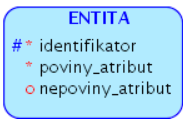
\includegraphics[width=0.25\textwidth]{topics/bi-wsi-si-02/images/entita.png}
\end{figure}

\subsection{Vztah 1:1, obě části jsou ve vztahu povinné}
Dojde k sjednocení daných entit do jedné tabulky
\textbf{zamestnanec\_vuz(\underline{cislo\_z}, jmneo\_z, adresa, spz, vyrobce, model)}.
Kde navíc \textbf{spz je NOT NULL a UNIQUE} (protože byl identifikátorem).
\begin{figure}[h!]
    \centering
    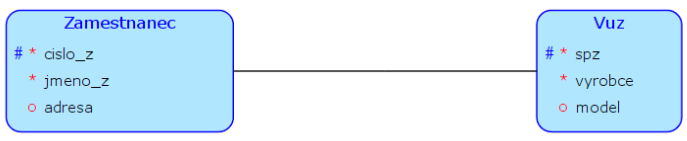
\includegraphics[width=0.5\textwidth]{topics/bi-wsi-si-02/images/oneToOne.png}
\end{figure}

\newpage

\subsection{Vztah 1:1, kde jen jedna část je povinná}
Entity se nemohou spojit kvůli nepovinnosti jedné strany. Převedou se tedy na dvě tabulky, kde tabulka, jež je nepovinnou částí, bude mít ID
odkaz na povinnou část.
\begin{figure}[h!]
    \centering
    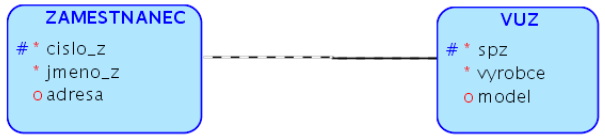
\includegraphics[width=0.5\textwidth]{topics/bi-wsi-si-02/images/oneToOneV2.png}
\end{figure}
\begin{itemize}
    \item zamestnanec(\underline{cislo\_z}, jmeno\_z, adresa)
    \item vuz(\underline{spz}, vyrobce, model, \texttt{cislo\_z}) a \underline{cislo\_z} je NOT NULL UNIQUE (kvůli zachování vazby 1:1)
    \item vuz[cislo\_z] $\subseteq$ zamestnanec[cislo\_z] 
\end{itemize}

\subsection{Vztah 1:1, obě nepovinné}
\begin{figure}[h!]
    \centering
    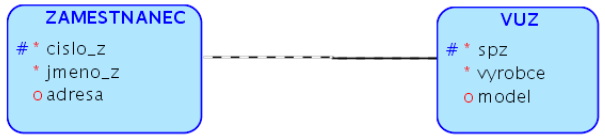
\includegraphics[width=0.5\textwidth]{topics/bi-wsi-si-02/images/oneToOneV2.png}
\end{figure}
Lze vyřešit dvěmi způsoby. \textbf{První řešení} odpovídá předchozímu případu, akorát \textbf{cislo\_z} v tabulce vuz bude \textbf{nepovinný}.

Druhé řešení přidává relační tabulky:
\begin{itemize}
    \item zamestnanec(\underline{cislo\_z}, jmeno\_z, adresa)
    \item vuz(\underline{spz}, vyrobce, model)
    \item zamestnanec\_vuz(\underline{cislo\_z}, spz), kde SPZ je NOT NULL a UNIQUE
    \item zamestnanec\_vuz[spz] $\subseteq$ vuz[spz]
    \item zamestnanec\_vuz[cislo\_z] $\subseteq$ zamestnanec[cislo\_z] 
\end{itemize}

\subsection{Vztah 1:N, povinná účást stany N (determinant)}
\begin{figure}[h!]
    \centering
    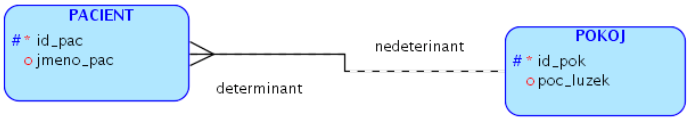
\includegraphics[width=0.6\textwidth]{topics/bi-wsi-si-02/images/oneToN.png}
\end{figure}
\begin{itemize}
    \item pacient(\underline{id\_pac}, jmeno\_pac, id\_pok)
    \item pokoj(\underline{id\_pok}, poc\_luzek)
    \item pacient[id\_pok] $\subseteq$ pokoj[id\_pok], kde id\_pok je NOT NULL
\end{itemize}


\subsection{Vztah 1:N, nepovinná účást stany N (determinant)}
Opět dva způsoby jak se dá řešit, první je vzít řešení z předchozí ukázky a nastavit \textbf{\underline{id\_pok} na nepovinný}. A druhé řešení
je opět vytvoření vazební tabulky
\begin{figure}[h!]
    \centering
    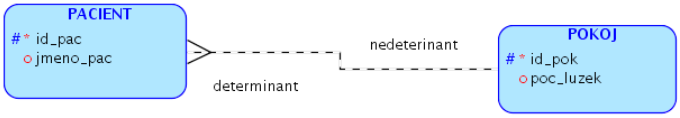
\includegraphics[width=0.6\textwidth]{topics/bi-wsi-si-02/images/oneToNV2.png}
\end{figure}
\begin{itemize}
    \item pacient(\underline{id\_pac}, jmeno\_pac),
    \item pokoj(\underline{id\_pok}, poc\_luzek)
    \item umisteni(\underline{id\_pac}, id\_pok), kde id\_pok je NOT NULL
    \item umisteni[id\_pac] $\subseteq$ pacient[id\_pac] 
    \item umisteni[id\_pok] $\subseteq$ pokoj[id\_pok]
\end{itemize}


\subsection{Vztah M:N}
\begin{figure}[h!]
    \centering
    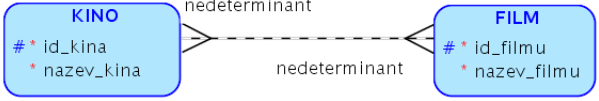
\includegraphics[width=0.6\textwidth]{topics/bi-wsi-si-02/images/MToN.png}
\end{figure}
\begin{itemize}
    \item kino(\underline{id\_kina}, nazev\_kina),
    \item film(\underline{id\_filmu}, nazev\_filmu)
    \item predstaveni(\underline{id\_kina, id\_filmu})
    \item predstaveni[id\_kina] $\subseteq$ kino[id\_kina]
    \item predstaveni[id\_filmu] $\subseteq$ film[id\_filmu]
\end{itemize}
Toto řešení způsobuje to, že v jendom kině se může hrát film pouze jednou. Tento problém se řeší pomocí dekompozice.

\subsection{Dekompozice vztahu M:N}
\begin{figure}[h!]
    \centering
    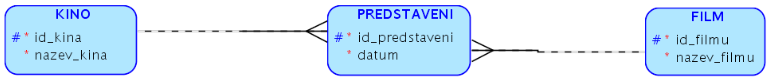
\includegraphics[width=0.8\textwidth]{topics/bi-wsi-si-02/images/decoMToN.png}
\end{figure}
\begin{itemize}
    \item kino(\underline{id\_kina}, nazev\_kina),
    \item film(\underline{id\_filmu}, nazev\_filmu)
    \item predstaveni(\underline{id\_predstaveni}, datum, id\_kina, id\_filmu), ID kina a filmu jsou NOT NULL
    \item predstaveni[id\_kina] $\subseteq$ kino[id\_kina] 
    \item predstaveni[id\_filmu] $\subseteq$ film[id\_filmu]
\end{itemize}


\subsection{Slabá entita}
Vezmeme v příklad čísla bloků a v jednotlivých blocích jsou pokoje. Bloky jsou číslované 1, 2,\dots,n a v každém bloku jsou číslované
pokoje od 1 do n. Pomocí samotného čísla pokoje se nedá identifikovat, kde se nachází, protože každý blok má pokoje stejně číslován.
Ale pomocí kombinace číslo bloku + číslo pokoje jsmě již schopní pokoj najít.
\begin{figure}[h!]
    \centering
    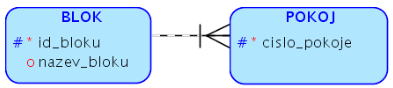
\includegraphics[width=0.4\textwidth]{topics/bi-wsi-si-02/images/weakEntity.png}
\end{figure}
\begin{itemize}
    \item blok(\underline{id\_bloku}, nazev\_bloku),
    \item pokoj(\underline{id\_pokoje, id\_bloku})
    \item pokoj[id\_bloku] $\subseteq$ blok[id\_bloku]
\end{itemize}

\subsection{Identifikační závislost}
\begin{figure}[h!]
    \centering
    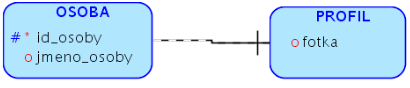
\includegraphics[width=0.4\textwidth]{topics/bi-wsi-si-02/images/idenRelation.png}
\end{figure}
Každý uživatel má pouze jeden profil a ten profil patří pouze jednomu uživateli. Uživatel nemusí mít profil, ale pokud ho má, tak je jasně
identifikován pomocí uživatele.
\begin{itemize}
    \item osoba(\underline{id\_osoby, jmeno\_osoby})
    \item profil(\underline{id\_osoby}, fotka)
    \item profil[id\_osoby] $\subseteq$ osoba[id\_osoby]
\end{itemize}

\section{ISA hierarchie}
Jedná se o způsob jak vyřešit více vztahů při převodu.
Rozdělují se na tři typy:
\begin{itemize}
    \item všechny vazby do jedné tabulky
    \item polymorfismus
    \item více oddělených tabulek
\end{itemize}
Příklad:
\begin{figure}[h!]
    \centering
    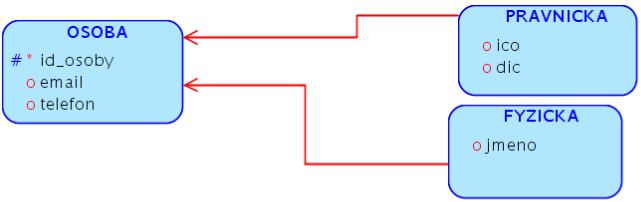
\includegraphics[width=0.7\textwidth]{topics/bi-wsi-si-02/images/isa.png}
\end{figure}
\begin{itemize}
    \item vše dohromady
    \begin{itemize}
        \item osoba(\underline{id\_osoby}, email, telefon, jmneo, ico, dic)
    \end{itemize}
    \item polymorfismus
    \begin{itemize}
        \item osoba(id\_osoby, email, telefon), kde ID osoby je UNIQUE
        \item fyzicka(\underline{id\_osoby}, jmneo)
        \item pravnicka(\underline{id\_osoby}, ico, dic)
        \item fyzicka[id\_osoby] $\subseteq$ osoba[id\_osoby]
        \item pravnicka[id\_osoby] $\subseteq$ osoba[id\_osoby]
    \end{itemize}
    \item oddělené tabulky
    \begin{itemize}
        \item fyzicka(\underline{id\_osoby}, email, telefon, jmneo)
        \item pravnicka(\underline{id\_osoby}, email, telefon, ico, dic)
    \end{itemize}
\end{itemize}
\end{document}